\section{Overview of $SPM_k$}

We begin this chapter by given a formal definition of $SPM$ and $SPM_k$.

\begin{mydef}
	\textbf{Shortest Path Map:} \\ 
	The shortest path map  of a
	particular source point s, denoted $SPM(s)$, is a subdivision of the plane
	into two-dimensional regions such that all the points in one region have the
	same, unique predecessor\cite{HershbergerS99}. In the case legal obstacle
	violations we use a shortest path map with k violations denoted by
	$SPM_k(p)$. This map has a fixed source and contains the set of unique
	shortest paths from $s$ to $p$, one for each number of violation we allow
	from $0,1,...,k$. 
\end{mydef}



\section{Algorithm for constructing $SPM_k$}

This section is dedicated to showing the extension of the Hershberger Suri algorithm which was presented in chapter 
\ref{chapter:conformingsubdivision} and \ref{chapter:shortestpathmap} for calculating a shortest $k$-path map, $SPM_k$ in time $O(k^2 \cdot 
n \log n)$. This is done by extending this continuous Dijkstra method into a $k$-garage structure. This way we can enter each level $i$ by 
going through an obstacle polygon in level $i-1$, and leave it into the next layer $i$. This can then be done up to $k$ times, which is 
equivalent to violating $k$ obstacles. So more precisely, when a wavefront hit an obstacle $O \in \mathcal{O}$, it claims the sub edges of 
the outer boundary of $O$, and then is re emitted into the interior of $O$, therefore also claiming the interior space of $O$. When reaching
the opposite side of $O$ from which it entered, it is re emitted into the free space free space a level higher than when entering. Therefore
this "vertical" movement in the interior of $O$ adds no time delay. So in this extension a wavefront at time $T$ contains all points at all 
levels which has $T$ distance to $s$. 

Another change has to be made to the Hershberger Suri algorithm which involves how we identifies generators i each level. Before we had a 
generator $g$ known by which vertex $v$ it start emitting from, and the time $t$ in which it starts to emit. When using the elevator we pass
through some subedges of $O$, which leads us to define the generators in term of a triplet, which now also involves the sub edge on the 
border of $O$ through which we enter this new level, see figure \ref{fig:tripletgenerator}.

\begin{figure}[H]
	\centering
	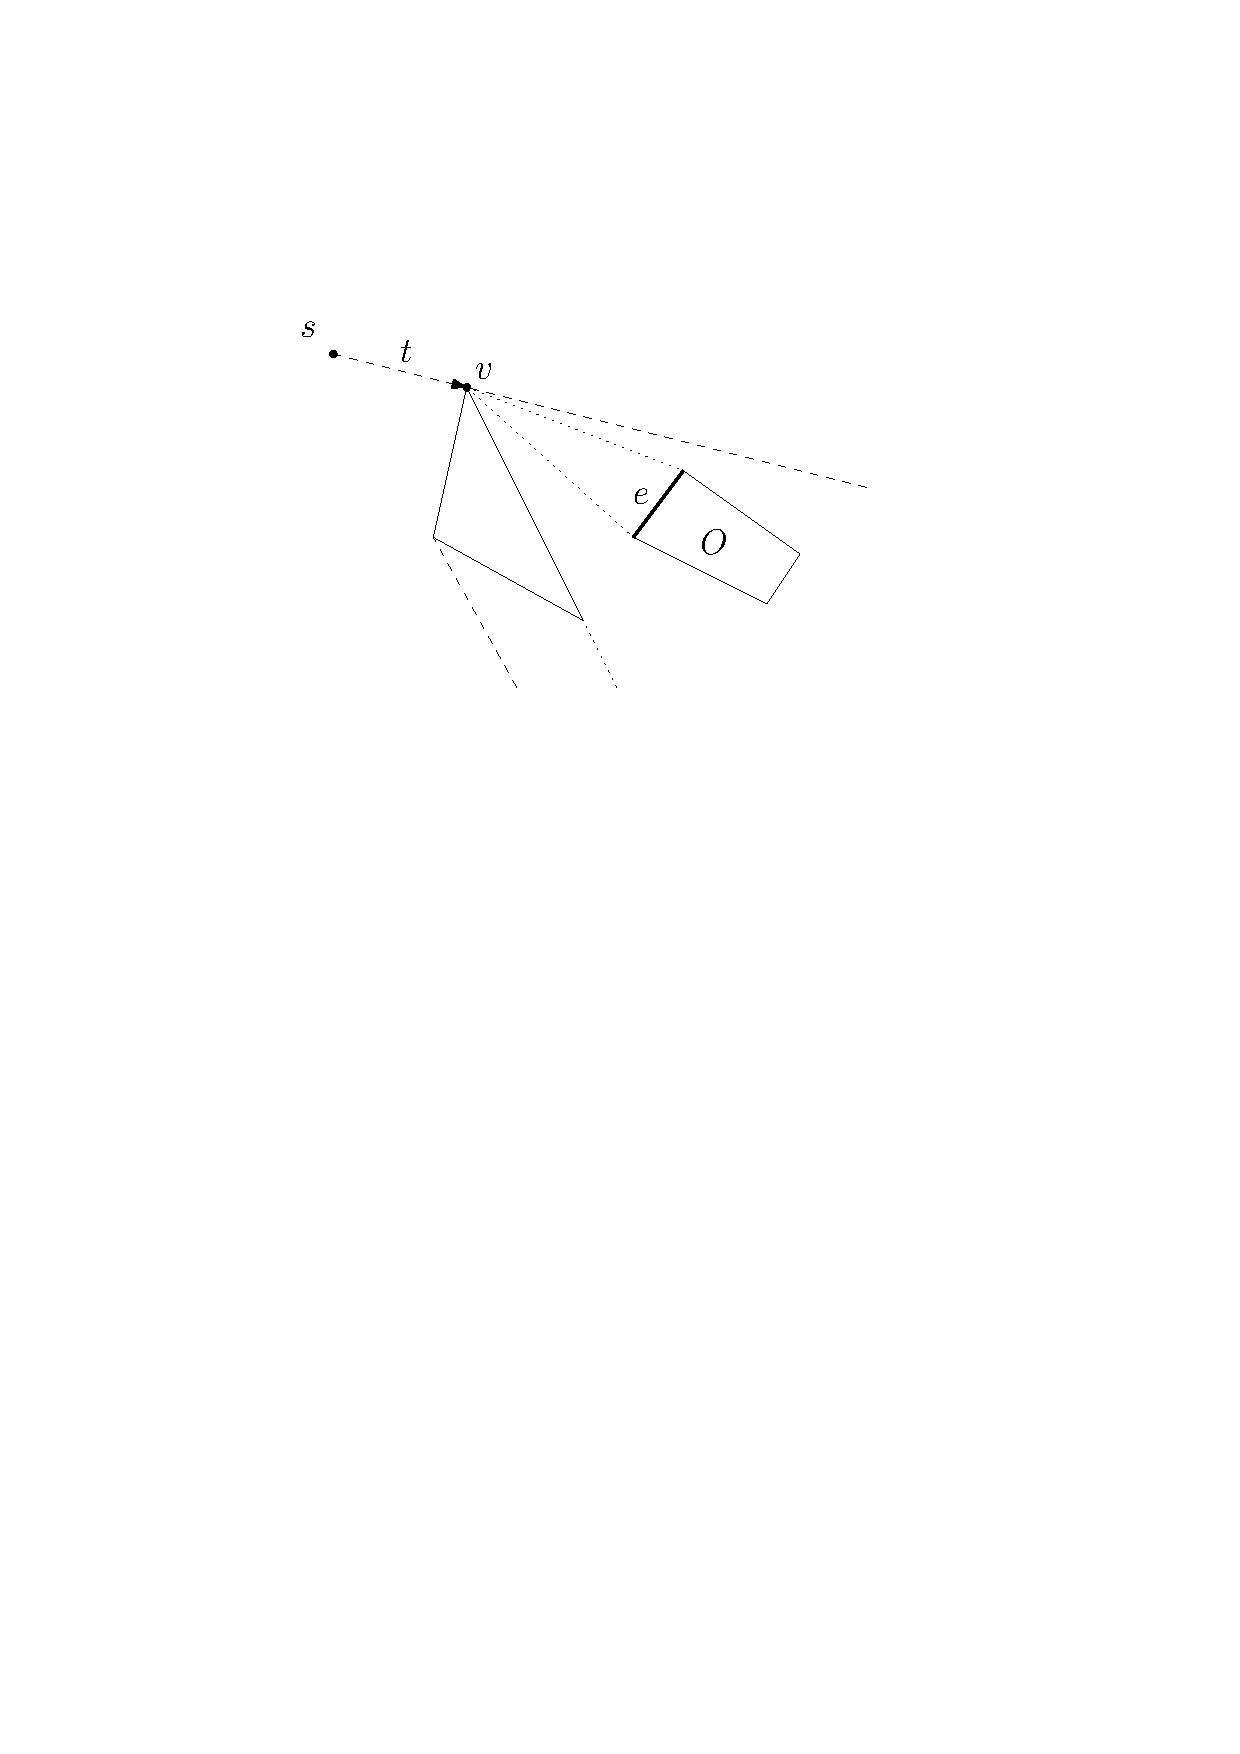
\includegraphics[width=0.8\textwidth]{figures/tripletgenerator.pdf}
	\caption{An example of a triplet generator where $v$ starts to emit at time $t$, and enter obstacle $O$ through edge $e$, which 
	         creates the new tiples generator $(v,t,e)$. }
	\label{fig:tripletgenerator}
\end{figure}

We can now imaging that entering the next level through $e$ is the same as emitting a wave from $v$ through the interior "triangular 
flap", shown in figure \ref{fig:tripletgenerator} with dotted lines, which is connected to $e$ and from there enter the free space at the 
next floor. Algorithmically we ignore the triangular flap, and start emitting directly from $e$, which is another difference compared to 
the unmodified Hershberger Suri algorithm where we only emitted from points, and not edges. So we do the following for each edge $e$ of 
the conforming sub division, as described in \cite{HershbergerKS17}:

\begin{enumerate}
    \item Find all boundary sources $(v,t,e)$ such that the well-covering region of $\mathcal{U}(f)$ which contains $e$.
    \item Initialize $covertime(f)$, which is the time at which $f$ would be engulfed by the wavefront minimizing over all boundary 
          sources $(v,t,e)$ with $e \in \mathcal{U}(f)$ and for each such source considering paths from $v$ with delay $t$, constrained to
          pass through $e$.
    \item For each source $(v,t,e)$ with $e \in \mathcal{U}(f)$, propagate its wavelet to $e$ inside $\mathcal{U}(f)$.
\end{enumerate}

By using the modified Hershberger Suri algorithm described above we get the following lemma, which we will use with out proof.

\begin{Lemma}[Lemma 22 in \cite{HershbergerKS17}]
Given $m$ boundary sources in a polygonal domain with $n$ vertices, we can compute the exit claims of the sources in $O((m + n) \cdot \log
(m + n))$ time and space.
\end{Lemma}

New we are ready to present the algorithm for constructing the $SPM_k$. The algorithm takes as a polygon $\mathcal{P}$ which encapsulate all 
the vertices in the plane we want in our $SPM_k$. The obstacles should be convex obstacles, which is a tighter condition than the unmodified 
Hershberger Suri algorithm, which also will work for non convex obstacles. Let $M$ denote the set of boundary sources, which will be 
passed to the modified Hershberger Suri algorithm. The algorithm computes two different things, namely the $(k-1)$-visibility region $V$ 
and the $k=$-path map $SPM_{=k}$, which together forms the $SPM_k$. The length from $s$ to a point $p$ in the plane by first locating the 
region in the $SPM_k$ which contains $p$ and then follow the $k$-predecessor of the region, back to $s$  adding their length.

\begin{algorithm}[H]
	\caption{Construct $SPM_k$} \label{algorithm:constructspmk}
	\begin{algorithmic}[1]
	    \State Set $M=\{s\}$
	    \State call the Hershberger-Suri algorithm on $\mathcal{P}$ and computer $SPM_0$
	    \State Let $V = \emptyset$
		\For {$i = 1$ to $k$}
		    \State \multiline{Using the modified Hershberger-Suri algorithm propagate the sources in $SPM_{i-1}$ the 
		                      obstacles in $\mathcal{P}$ and compute the set of boundary sources $M_{new}$ for $SPM_{=i}$}
            \State \multiline{Identify all the regions in $SPM_{=(i-1)}$ for which the predecessor is $s$. Observe 
                             that this is precisely the region $V' = V_{i-1} \setminus V_{i-2}$. Set $\mathcal{P}$ to be the 
                             new polygon domain with this region removed.}
            \If {$V = \emptyset$ then}
                \State {set $V = V'$}
            \Else 
                \State {Merge $V$ with $V'$ at the common vertices.}
            \EndIf
            \State {Set $M = M_{new}$}
            \State \multiline{Call the modified Hershberger-Suri algorithm  to compute $SPM_{=i}$ for input $P$}
        \EndFor
        \State \multiline{Merge $SPM_{=k}$ with $v$ at the boundary of regions of $SPM_{=k}$ that have $s$ as predecessor, 
                          i.e. $V' = V_k \setminus V_{k-1}$ to obtain $SPM_k$}
	\end{algorithmic} 
\end{algorithm}

When end this chapter with the theorem for the running time of algorithm above

\begin{theorem} [Theorem 23 in \cite{HershbergerKS17}]
If $P$ is a polygonal domain bounded by convex obstacles with a total of $n$ vertices, the shortest $k$-path map for $P$ with respect to a srouce point $s$ can be computed in $O(k^2 \cdot n \cdot \log n)$ time and $O(k \cdot n \log n)$ space.
\end{theorem}
